
    
    % !TEX encoding = UTF-8 Unicode
    
    
    
    
    \documentclass[conference,compsoc]{IEEEtran}
    
    \usepackage{graphicx}
    \usepackage{epstopdf}
    \DeclareGraphicsExtensions{.eps}
    \usepackage{url}
    \usepackage{multicol}
    
    
    
    
    
    
    
    \ifCLASSOPTIONcompsoc
    
      \usepackage[nocompress]{cite}
    \else
      % normal IEEE
      \usepackage{cite}
    \fi
    
    \ifCLASSINFOpdf
    
    \else
    
    \fi
    
    
        
    % correct bad hyphenation here
    \hyphenation{op-tical net-works semi-conduc-tor}
    
    \usepackage[utf8x]{inputenc} 
    
    \usepackage{array}
    \newcolumntype{L}[1]{>{\raggedright\let\newline\\\arraybackslash\hspace{0pt}}m{#1}}
    \newcolumntype{C}[1]{>{\centering\let\newline\\\arraybackslash\hspace{0pt}}m{#1}}
    \newcolumntype{R}[1]{>{\raggedleft\let\newline\\\arraybackslash\hspace{0pt}}m{#1}}
    
    \usepackage{float}
    \usepackage{listings}
    
    
    \begin{document}
    %
    % paper title
    % Titles are generally capitalized except for words such as a, an, and, as,
    % at, but, by, for, in, nor, of, on, or, the, to and up, which are usually
    % not capitalized unless they are the first or last word of the title.
    % Linebreaks \\ can be used within to get better formatting as desired.
    % Do not put math or special symbols in the title.
    \title{Study of QoS and Traffic Control Mechanisms in IP Networks}
    
    % author names and affiliations
    % use a multiple column layout for up to three different
    % affiliations
    \author{\IEEEauthorblockN{Filipe Oliveira, João Rua, Miguel Zenha}
    \IEEEauthorblockA{Computer Science Department\\
    Universidade do Minho\\
    Email: a57816@alunos.uminho.pt, a41841@alunos.uminho.pt, a66551@alunos.uminho.pt,}
    }
    
    % make the title area
    \maketitle
    
    % As a general rule, do not put math, special symbols or citations
    % in the abstract
    \begin{abstract}
    In traditional networks, all connections and services get the same treatment. However, since network resources are limited, and the overall Internet only offers a "Best-Effort" approach, it is important to differentiate between connection classes, and to be able to treat them accordingly to standardised and well documented parameters. \par 
    This exploratory essay focus on developing a comparative study of traffic control mechanisms in IP networks and corresponding parametrisation,
    using the Network Simulator NS-2. In order to do so, a test platform will be presented and several Diffserv parameters will be discussed.
    \end{abstract}
    
    \IEEEpeerreviewmaketitle
    
    \section{Network topology to be used}
    
    The network topology to be used as test platform is illustrated in figure \ref{fig:network}. The network topology includes six clients (from Cli1 to Cli6), two edge routers (E1 and E2), and a core router (C0). The clients' access links have a capacity of 5Mbps and a delay of 5ms, and the core network links have a capacity of 5Mbps and a delay of 10ms.\par 
    
    \begin{figure}[H]
    \centering
    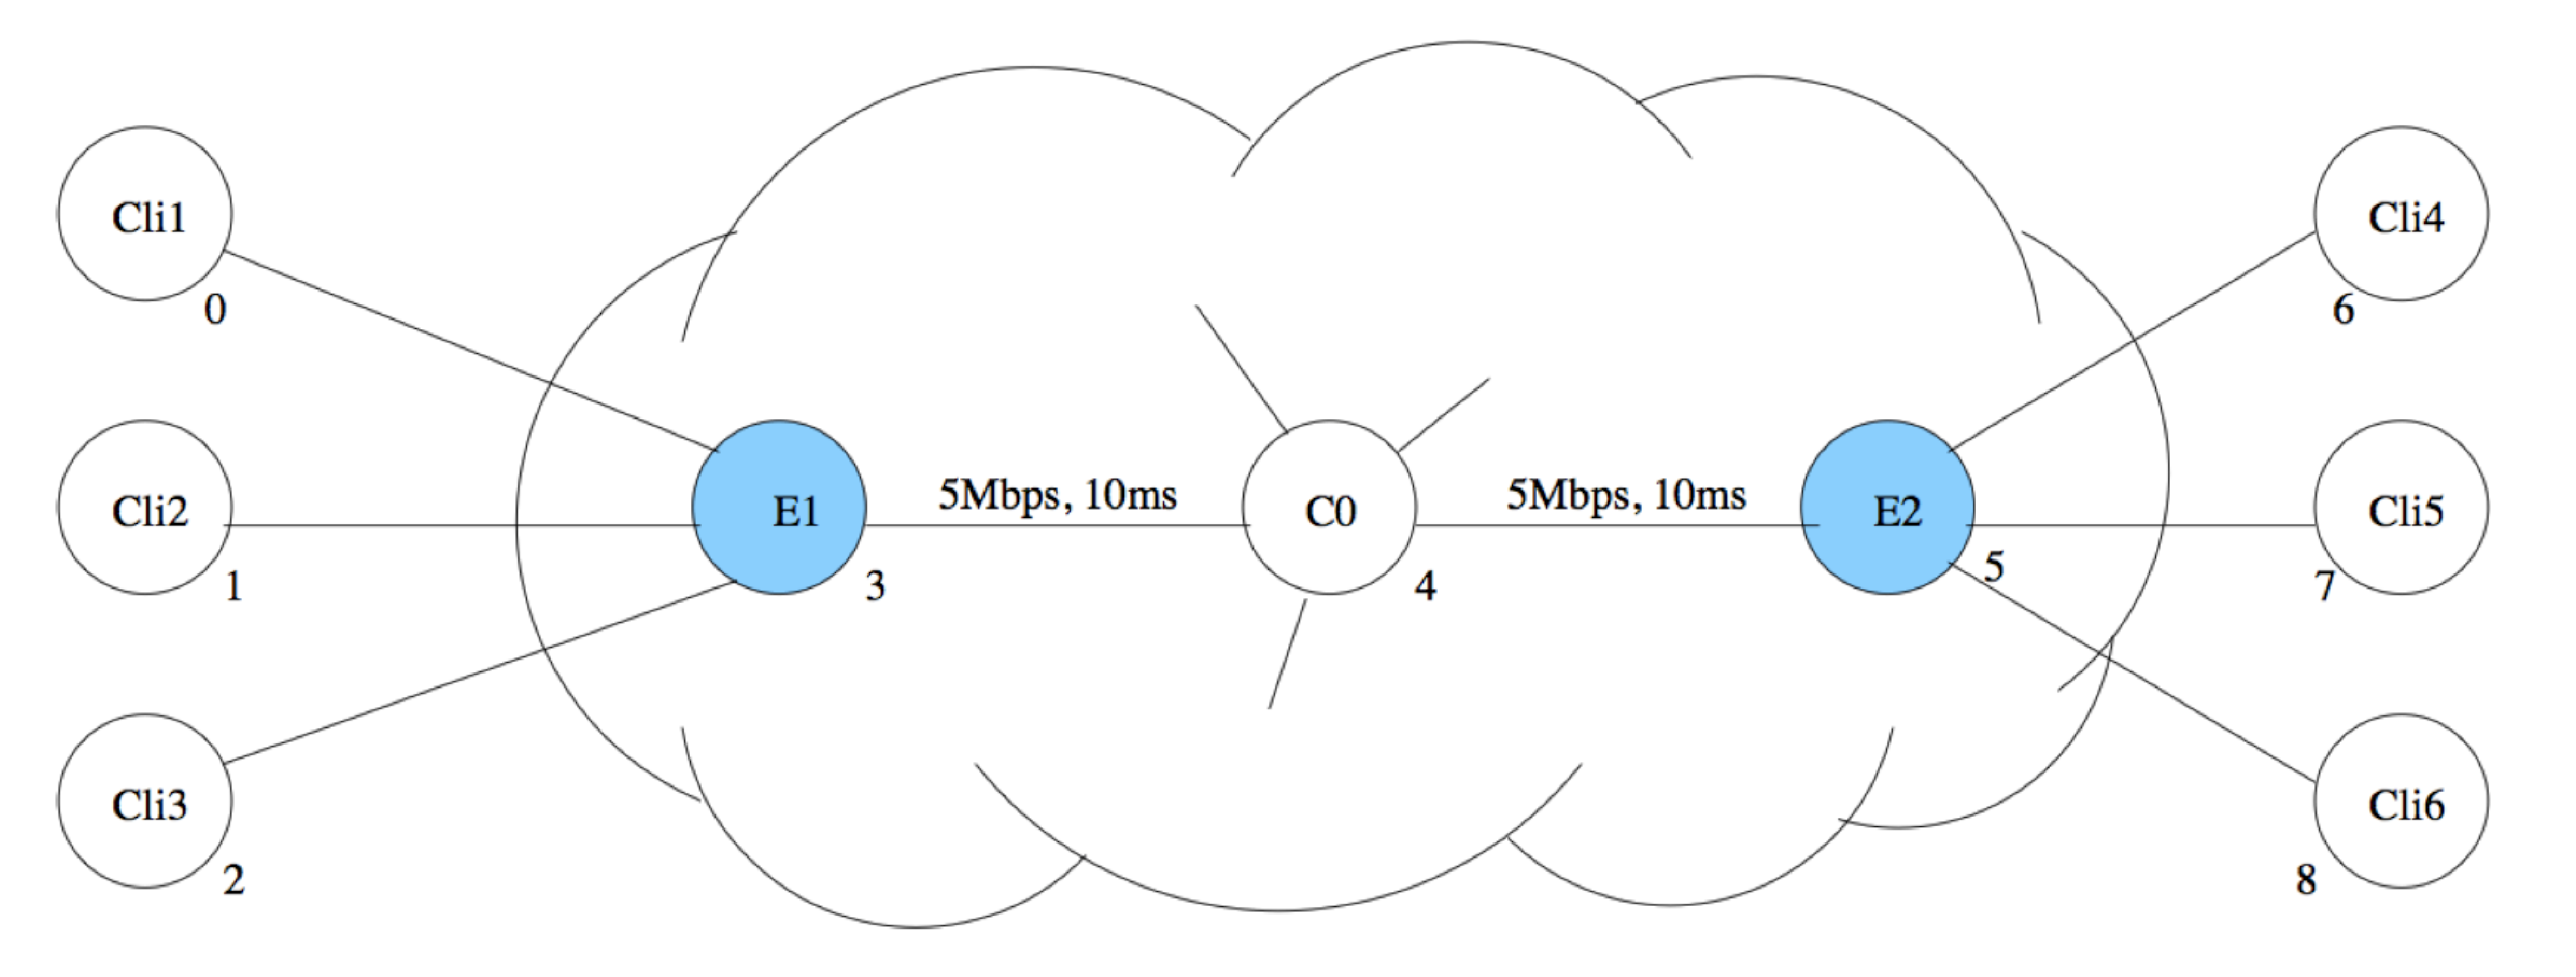
\includegraphics[width=1\columnwidth]{PNG/network.png}
    \caption{ISP network topology}
    \label{fig:network}
    \end{figure}
    
    The topology is deliberately symmetric to simplify traffic analysis.
    During this exploratory essay several changes will be made regarding the services/applications that every Client holds, however, the topology remains unchanged. \par 
    In most of the cases, it will be enough to analyse flow in one way, however, in the last analyse on chapter \ref{c5}, flows in both ways will be analysed due to the bigger complexity of the simulation.\par 
    As the topology evidences, if all clients use the link capacity simultaneously then congestion will occur in the network backbone, and the service provider will not be able to guarantee proper traffic delivery. To minimise or solve this effect, several traffic control mechanisms will be used in order to promote quality of service (QoS) in the domain.\par 
    Simulations for all scenarios were 15 seconds long. This was a very short simulation time, but enabled us to achieve a confidence interval, producing a stable final state.
    
    \section{Applications/Services to be used}
    
    \begin{itemize}
        \item \textbf{CBR over UDP} - generates Constant Bit Rate (CBR) traffic over UDP. This may correspond to
    the transmission of audio or video traffic at a regular/periodic rate.
    \begin{itemize}
        \item Parameters: rate (bits/sec) e packet size (Bytes);
    \end{itemize}
        \item \textbf{FTP} - transfer of large files over TCP;
        \item \textbf{Voice over UDP} - simulates a voice call over UDP; This traffic is characterised by having a constant
    rate, alternating between talk and silence time periods.
    \begin{itemize}
        \item Parameters: rate (bits/sec) and burst size (in seconds).
    \end{itemize}
    \end{itemize}
    
    
    \section{Tools and evaluation metrics}
    In order to infer the network quality of service we will take in consideration the following parameters 
    Metrics to use in the simulations:
    \begin{itemize}
        \item \textbf{Loss rate} (total and per flow), in packets/sec.
        \item \textbf{Bandwidth} in use (total and per flow), in bits/sec.
    \end{itemize}
    
    \section{A - Simulating the "Best-Effort" scenario}
    
    By default, routers handle packets based on a simple FIFO queueing system, trying to forward them in
    the best possible way according to the available resources (memory and CPU). \par This well-known model is called Best-Effort as there are \textbfno QoS guarantees} on packet delivery (in terms of bounded delays, loss
    and/or bandwidth utilisation). \par 
    For a first approach we considered similar clients with CBR applications,  generating each one a rate of 3Mbps, for a total of six flows (0 $ \rightarrow $ 8, 1 $ \rightarrow $ 7, 2 $ \rightarrow $ 6, 8 $ \rightarrow $0, 7 $ \rightarrow $1,
    6 $ \rightarrow $2).\par 
    
    \subsection{Identification of the links under congestion}
    
    Producing the graphs illustrating the levels of loss and bandwidth
    utilisation along the time, we can infer that the core network links ( 3 $ \leftrightarrow $ 4, 4 $ \leftrightarrow $ 5 ), since the full bandwidth is being used, as stated in figures \ref{graph:bw_a2} and \ref{graph:loss_a2}.
    
    \begin{figure}[H]
    \centering
    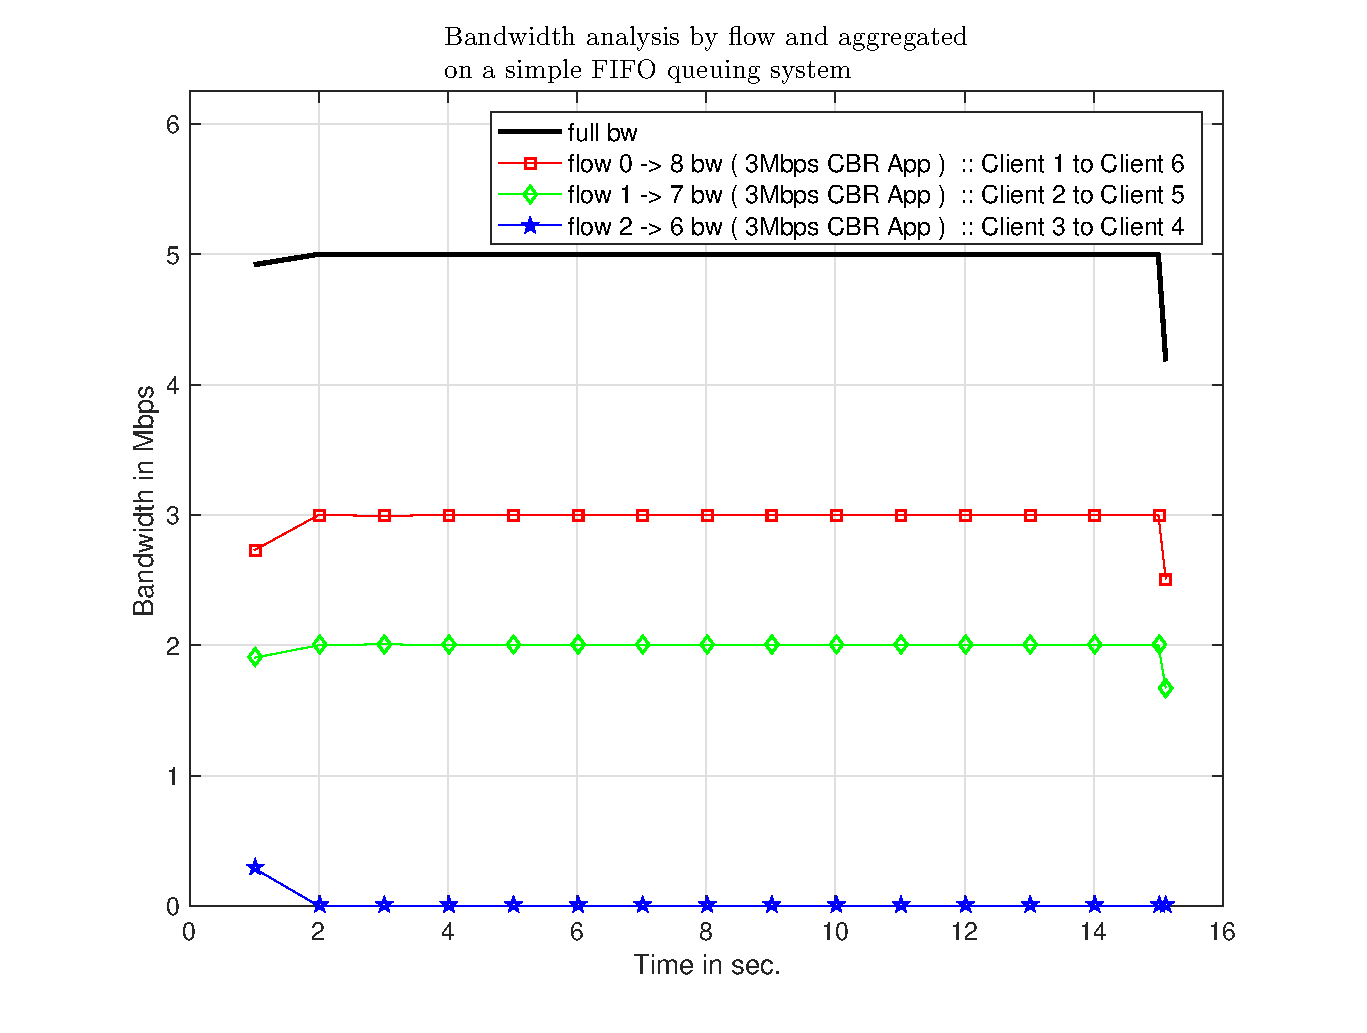
\includegraphics[width=1\columnwidth]{EPS/A/bw_a2.eps}
    \caption{Bandwidth analysis by flow and aggregated on a simple FIFO queueing system, simulation a "best effort" scenario}
    \label{graph:bw_a2}
    \end{figure}
    
    
    \begin{figure}[H]
    \centering
    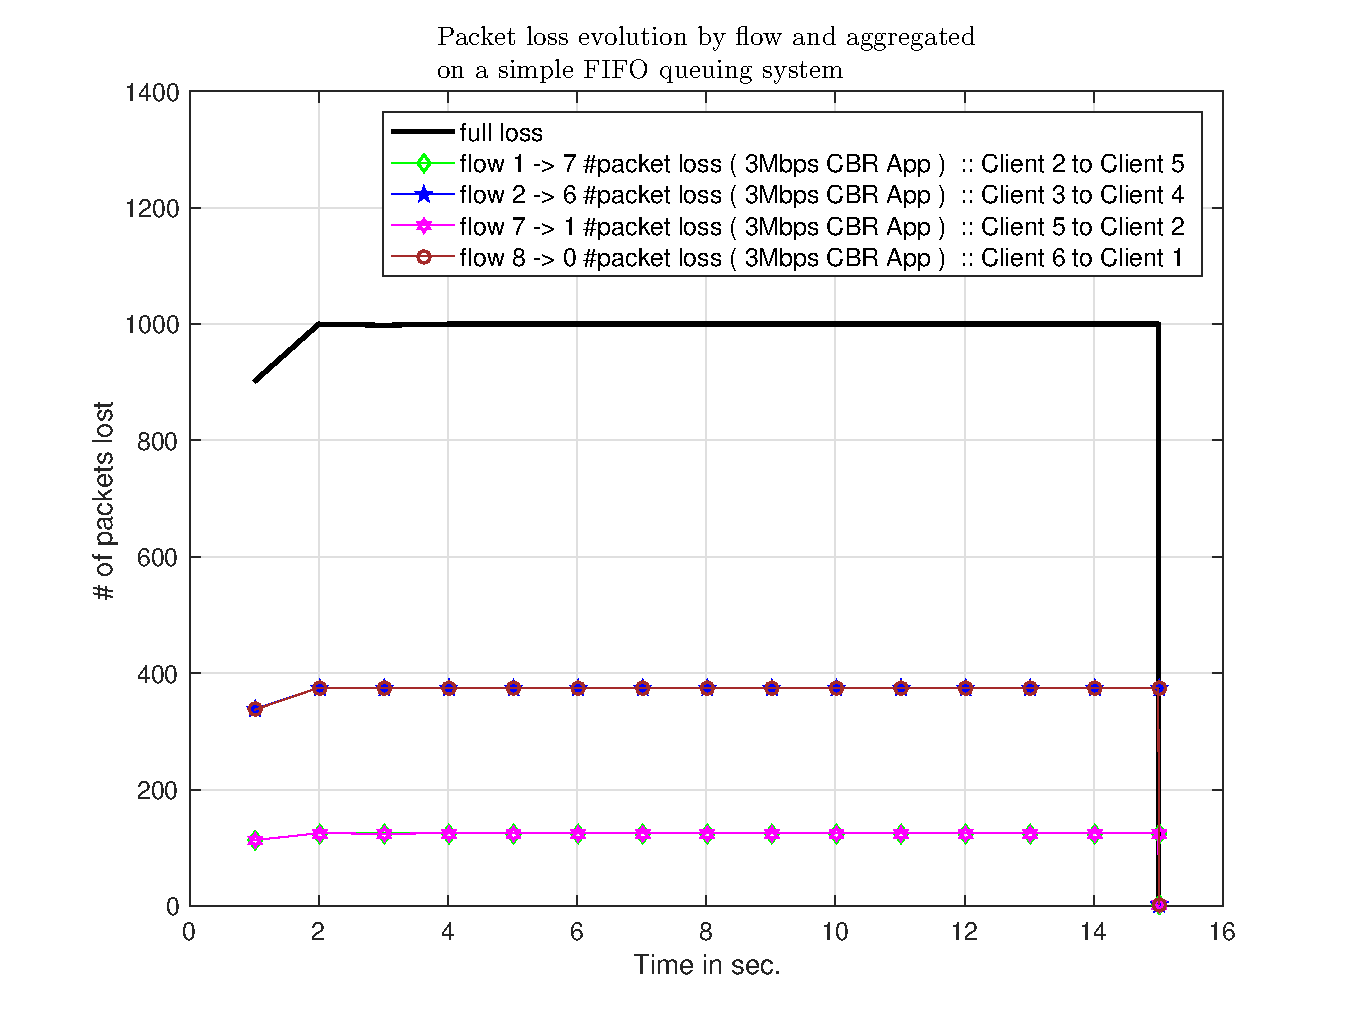
\includegraphics[width=1\columnwidth]{EPS/A/loss_a2.eps}
    \caption{Packet loss evolution by flow and aggregated on a simple FIFO queueing system, simulation a "best effort" scenario}\label{graph:loss_a2}
    \end{figure}
    
    As stated before, the Internet's "best-effort" scenario produces an undesired non-equitable bandwidth distribution. Denote that this simple simulation only deals with one type of service simulation. The inclusion of other, "more sensible" to network congestion, services like for example VOIP, would result in an unacceptable QoS.\par
    Changing the queues associated with the links under congestion from DropTail to RED would theoretically result into in a better service. The corresponding results are shown in figures \ref{graph:bw_a2_red} and \ref{graph:loss_a2_red}.
    
    \begin{figure}[H]
    \centering
    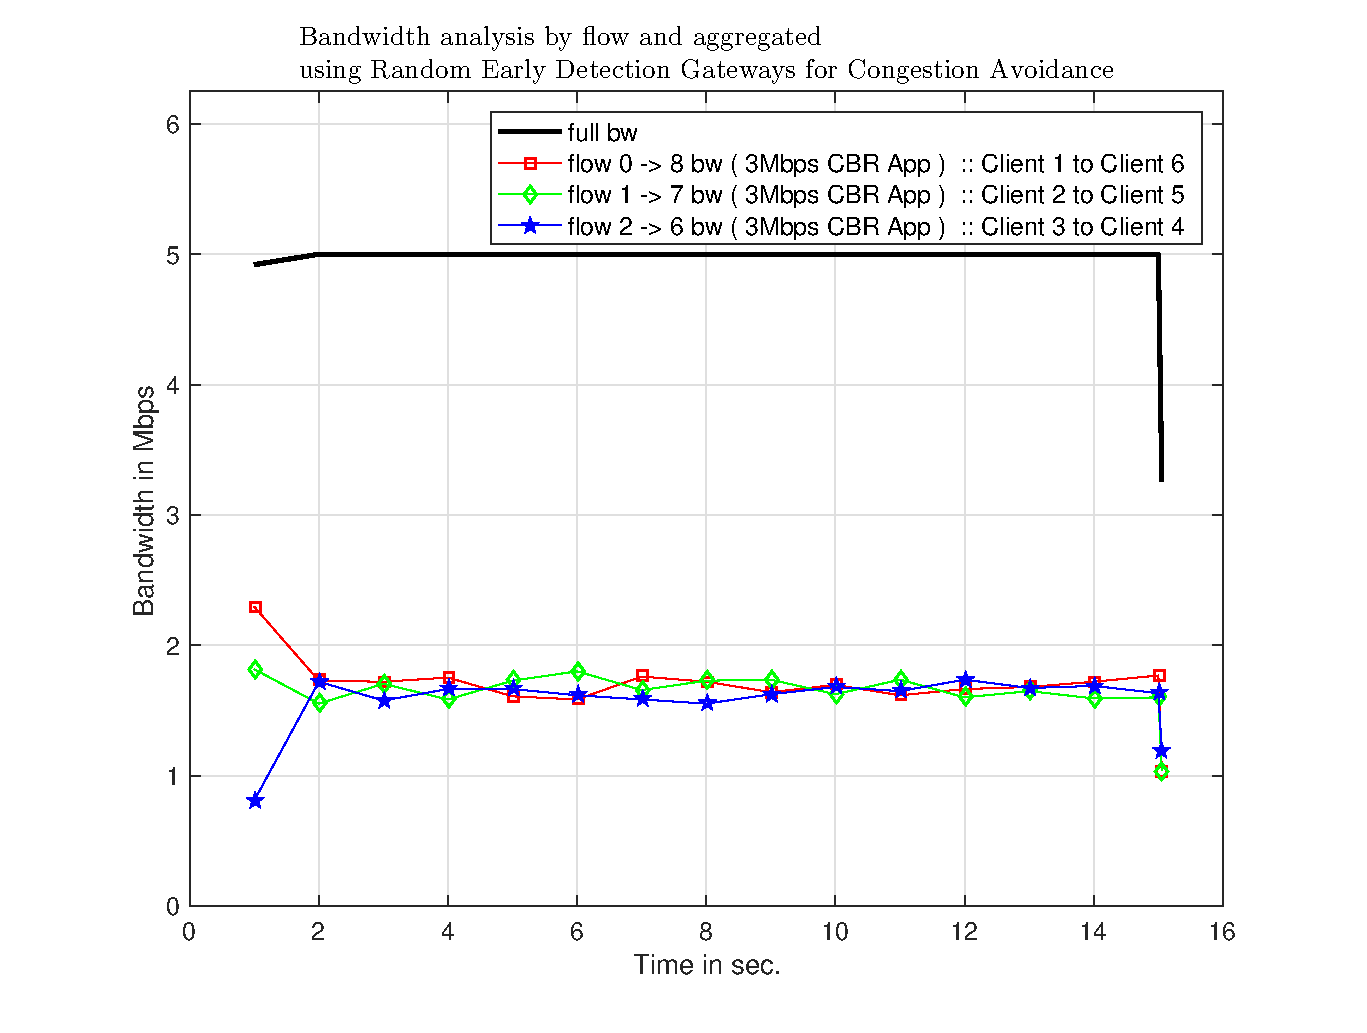
\includegraphics[width=1\columnwidth]{EPS/A/bw_a2_red.eps}
    \caption{Bandwidth analysis by flow and aggregated on a simple FIFO queueing system, simulation a "best effort" scenario, using Random Early Detection Gateways for Congestion Avoidance}
    \label{graph:bw_a2_red}
    \end{figure}
    
    
    \begin{figure}[H]
    \centering
    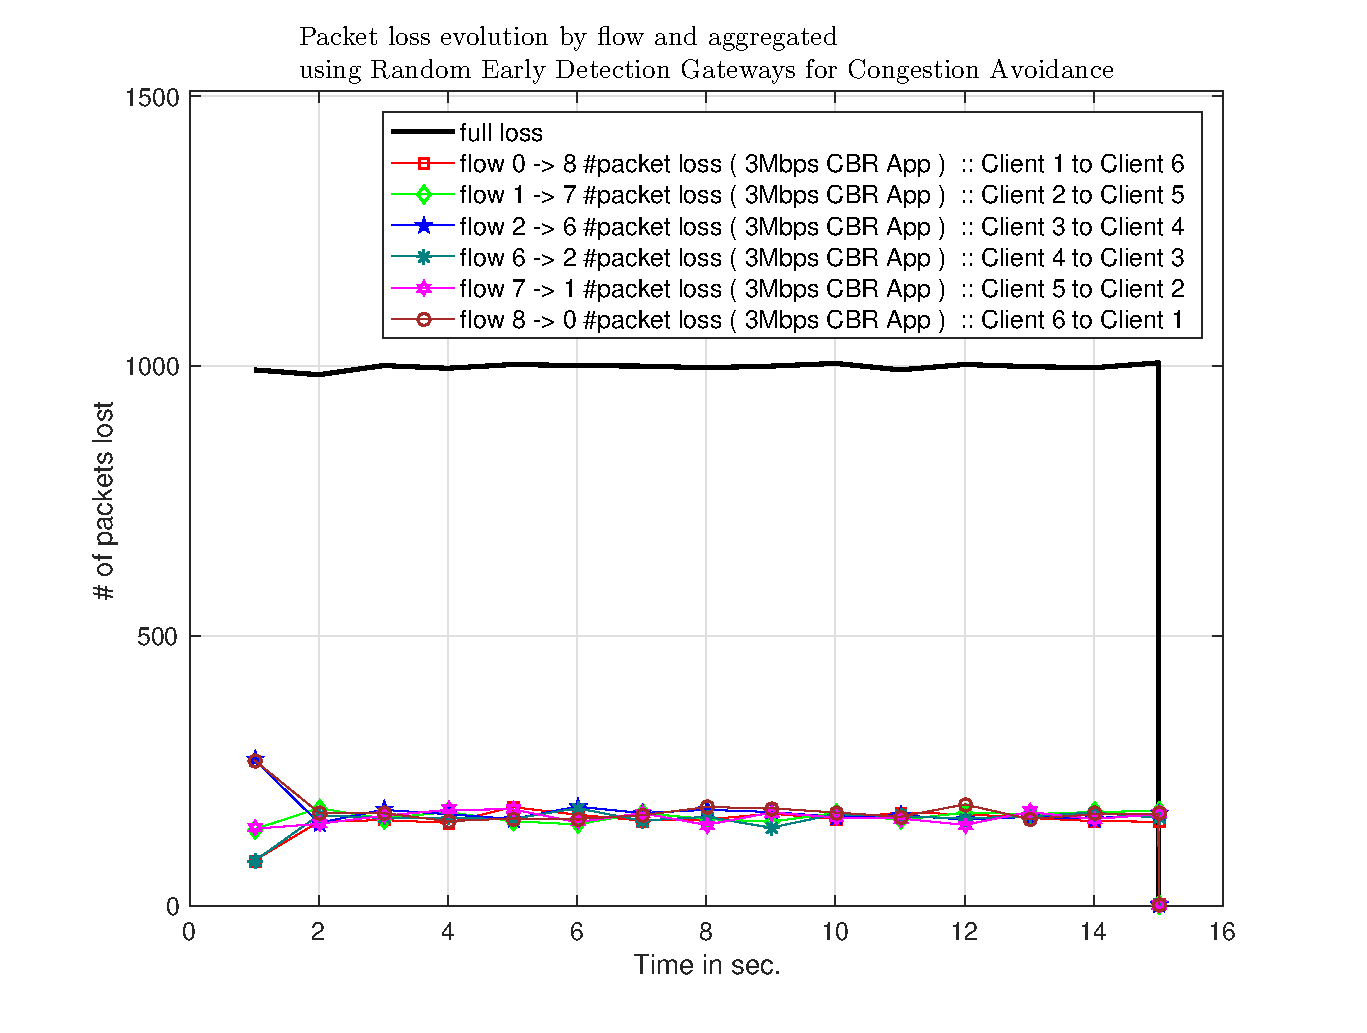
\includegraphics[width=1\columnwidth]{EPS/A/loss_a2_red.eps}
    \caption{Packet loss evolution by flow and aggregated on a simple FIFO queueing system, simulation a "best effort" scenario, using Random Early Detection Gateways for Congestion Avoidance}\label{graph:loss_a2_red}
    \end{figure}
    
    Notice that this "solution" only improves the equitable bandwidth distribution across flow because they all are produced with the same service/traffic type. If we included for exemplo some TCP over IP service, since it behaves in order to prevent/diminish congestion, it would suffer more from  bandwidth "starvation" than any service using UDP over IP. \par
    In figures   \ref{graph:bw_a3} and \ref{graph:loss_a3}, simulated results are show if one client would generate more CBR traffic than
the others, on a simple FIFO queuing system, simulating a "best effort" scenario.

  \begin{figure}[H]
    \centering
    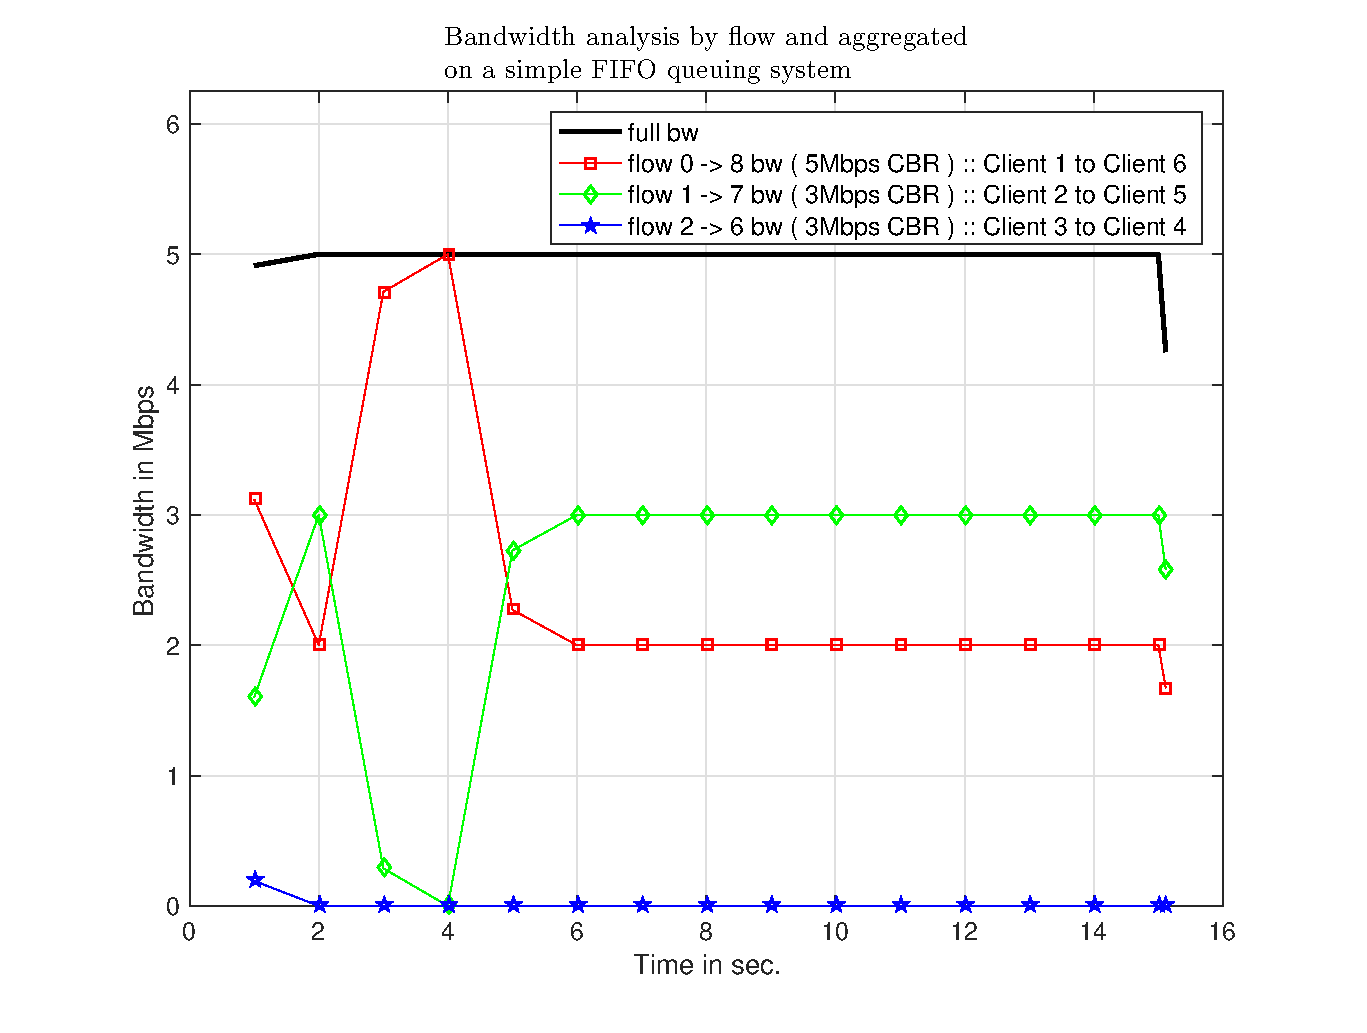
\includegraphics[width=1\columnwidth]{EPS/A/bw_a3.eps}
    \caption{Bandwidth analysis by flow and aggregated on a simple FIFO queueing system, simulation a "best effort" scenario,  in which one client would generate more CBR traffic than the others.
the others}
    \label{graph:bw_a3}
    \end{figure}
    
    
    \begin{figure}[H]
    \centering
    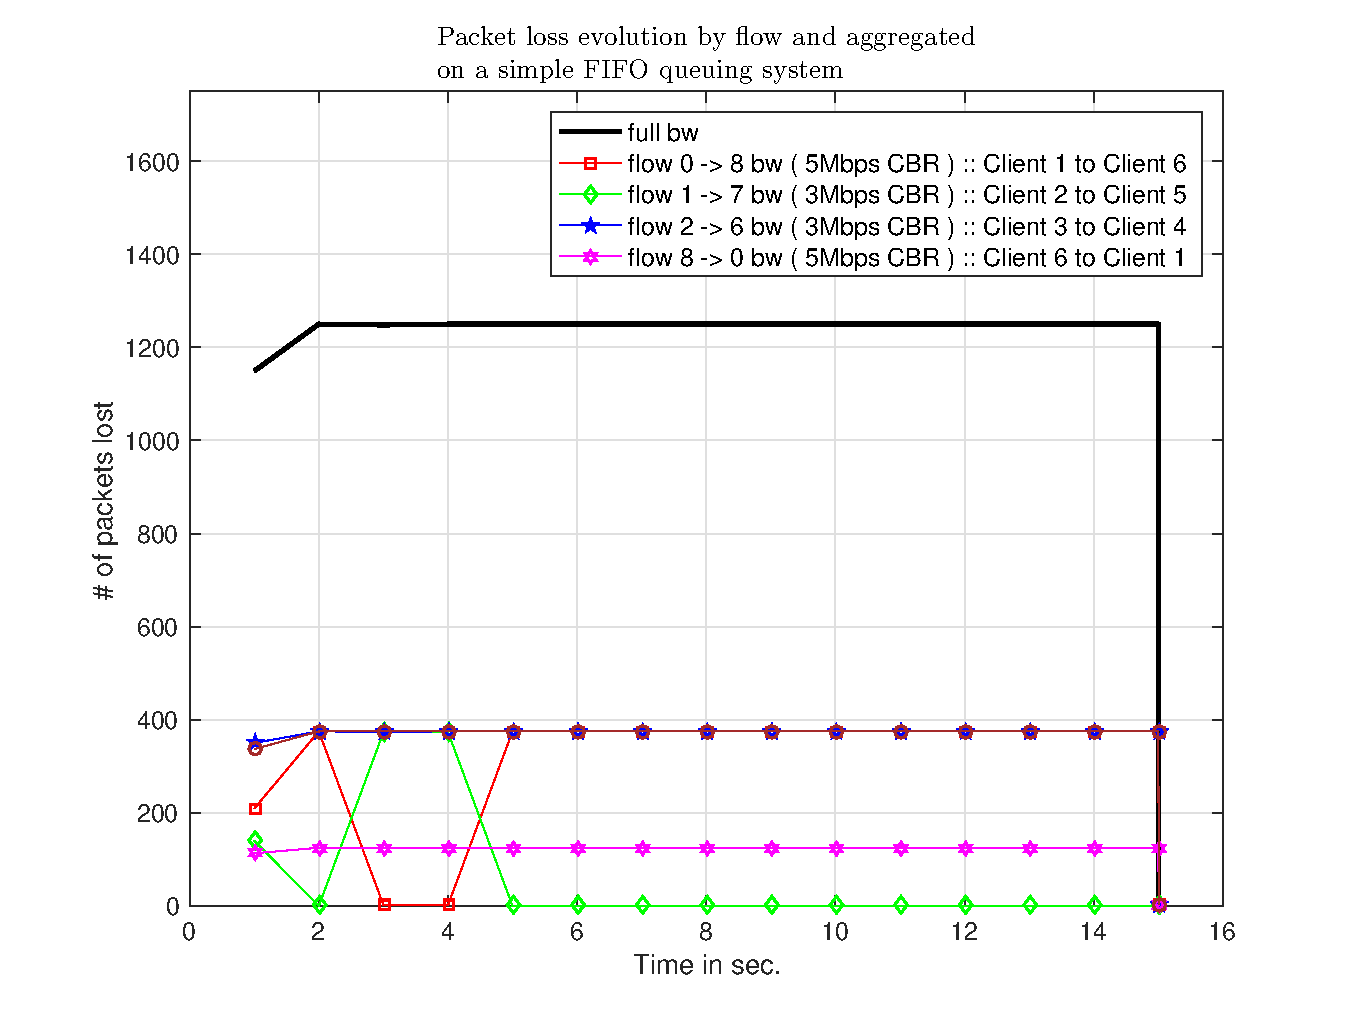
\includegraphics[width=1\columnwidth]{EPS/A/loss_a3.eps}
    \caption{Packet loss evolution by flow and aggregated on a simple FIFO queueing system, simulation a "best effort" scenario,  in which one client would generate more CBR traffic than the others.
    
the others}\label{graph:loss_a3}
    \end{figure}
    
    
     \section{B - Simulating a multi-service network in  the "Best-Effort" scenario}


In a more realistic scenario, it would be expectable to have both UDP and TCP traffic with other characteristics (FTP, HTTP, etc.).
Using the procedures already included in the simulation script, several changes were made in order to obtain the
following scenario:
\begin{itemize}
\item \textbf{a CBR application} sending 4Mbps from client 1 to client 6, and other from client 6 to client 1;
\item  \textbf{a FTP connection} from client 2 to client 5, and other from client 4 to client 2;
\item  \textbf{a voice connection over UDP} from client 3 to client 4, and vice-versa. Since VOIP Bandwidth consumption naturally depends on the codec used, we selected G.711 - 64 Kbps Bitrate and 87.2 Kbps Nominal Ethernet Bandwidth, and simulated a maximum of 30 calls at any given simulation time. The presented graphic results for VOIP are a aggregation of all the 30calls. 
\end{itemize}
The corresponding results are shown in figures \ref{graph:bw_b1} and \ref{graph:loss_b11}.

  \begin{figure}[H]
    \centering
    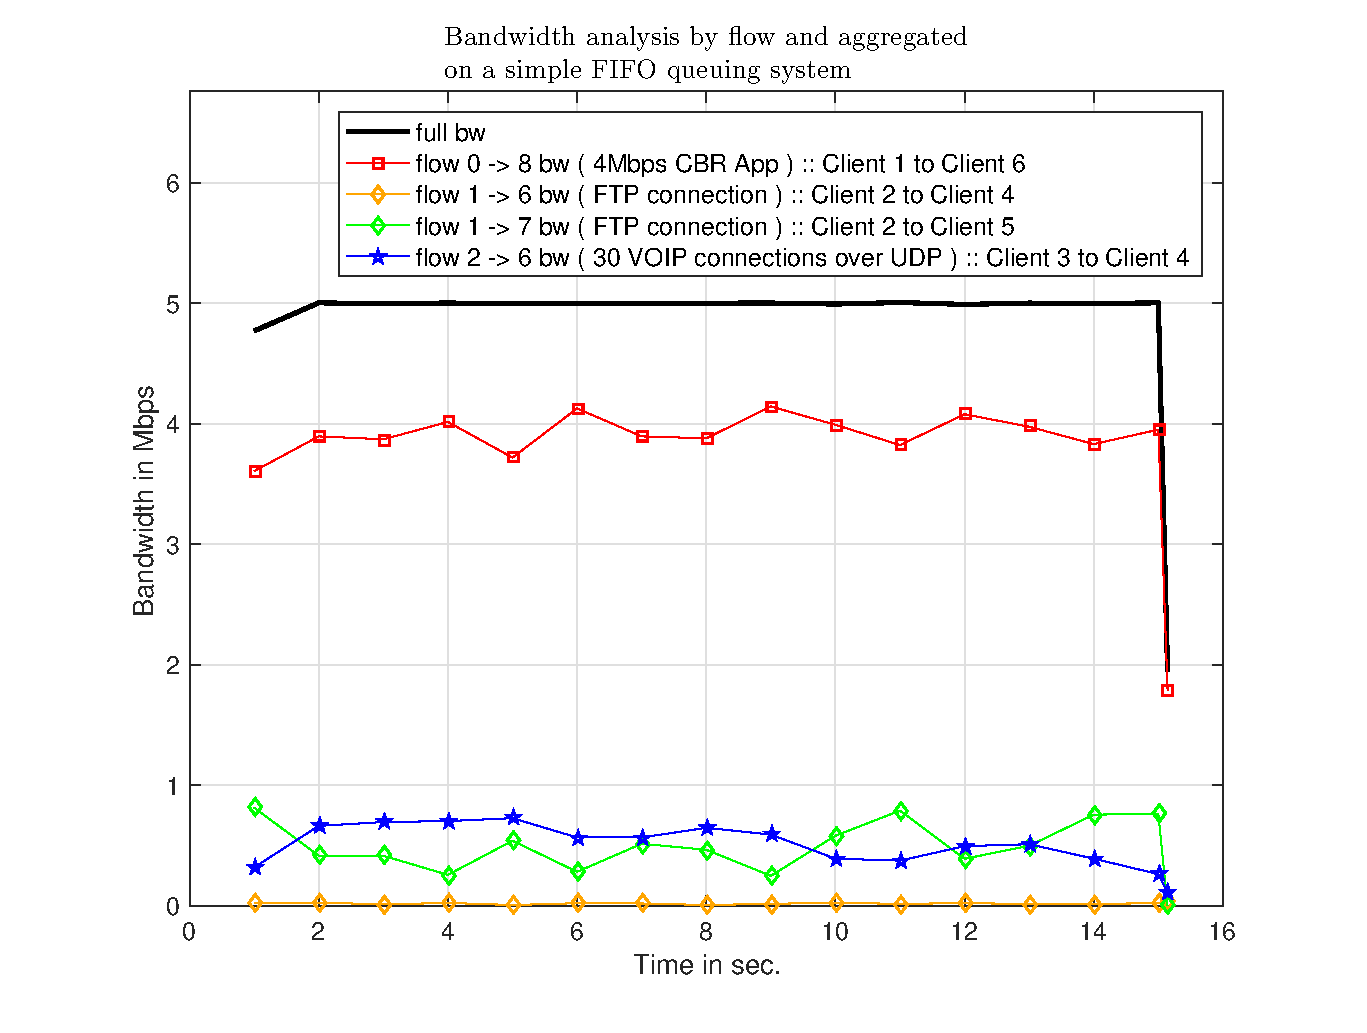
\includegraphics[width=1\columnwidth]{EPS/B/bw_b1.eps}
    \caption{Bandwidth analysis by flow and aggregated on a simple FIFO queueing system, simulating a multi-service network in a "best effort" scenario,  on a simple FIFO queuing system.}
    \label{graph:bw_b1}
    \end{figure}
    
    
    \begin{figure}[H]
    \centering
    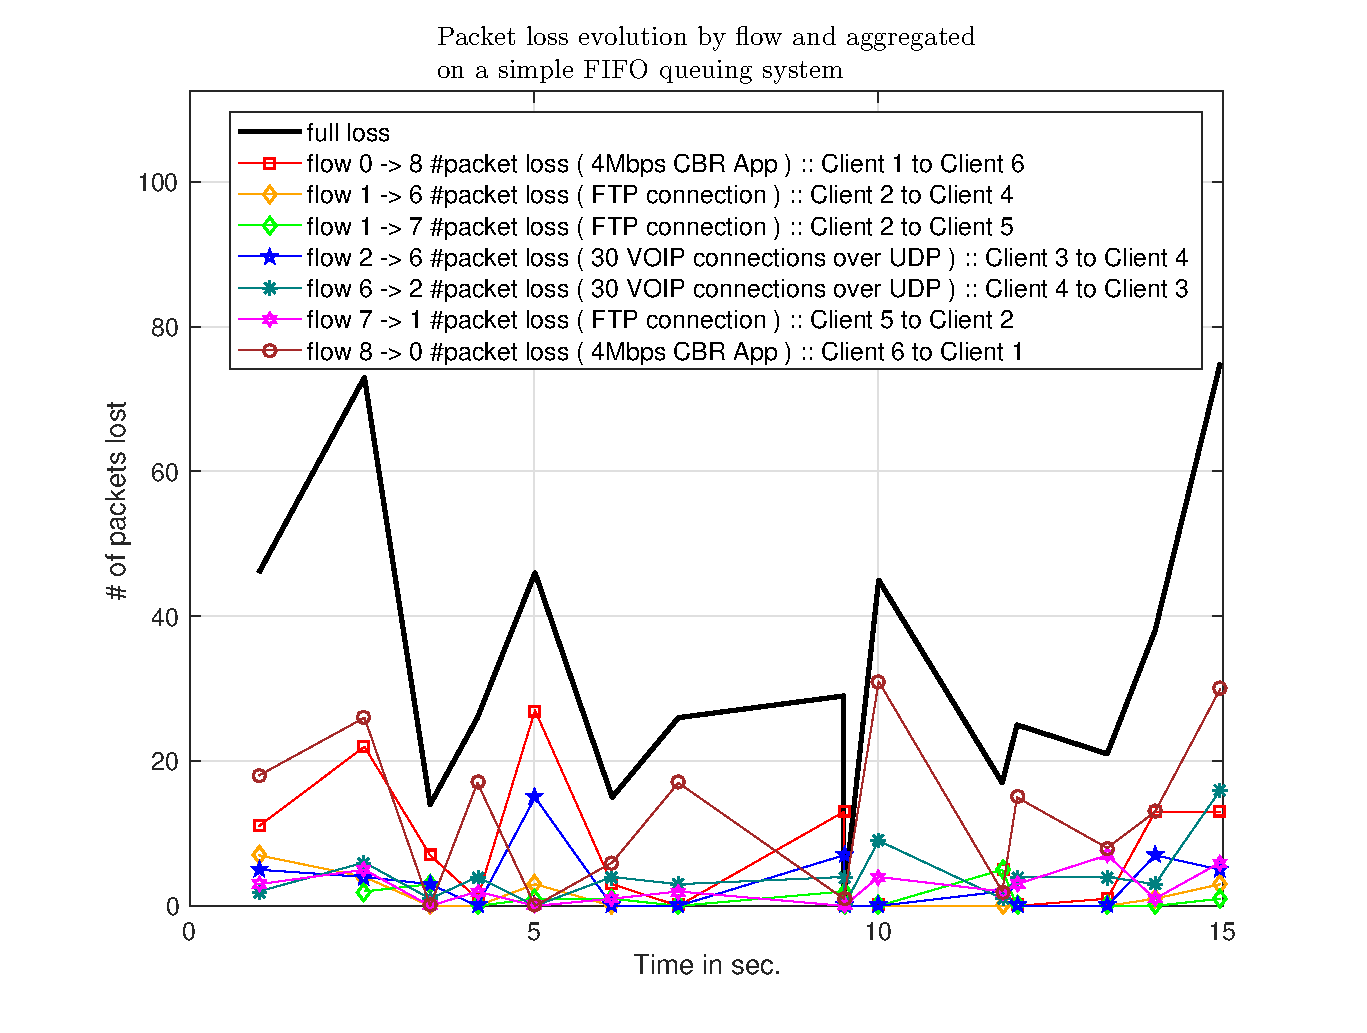
\includegraphics[width=1\columnwidth]{EPS/B/loss_b1.eps}
    \caption{Packet loss evolution by flow and aggregated on a simple FIFO queueing system, simulating a multi-service network in a "best effort" scenario,  on a simple FIFO queuing system.}
\label{graph:loss_b11}
    \end{figure}

    
    \section{C.1 Identify the links under congestion}
    
    \subsection{E1 - C0 (Edge to Core Configuration)}
    \begin{itemize}
        \item \textbf{The number of existing queues and the traffic scheduler in use} \par 
        1 physical queue,  implementing 2 virtual queues;  
        \vspace{5mm}
        \item \textbf{Policy Entry}
        \begin{itemize}
            \item \textbf{Client1 $\rightarrow$ Client6} -- TokenBucket:
            \begin{itemize}
                \item \textbf{Committed Information Rate:} 2 Mbits/sec;
                \item \textbf{Committed Burst Size:} 5 KBytes;
                \item \textbf{Policer Table} has initial (green) code point 10, and downgraded (yellow) code point 11;
            \end{itemize}
            \item \textbf{Every remaining initial and end station} -- Dumb:
             \begin{itemize}
                \item \textbf{Policer Table} has always downgraded (yellow) code point 11;
            \end{itemize}
        \end{itemize}
        
        \vspace{5mm}
        \item \textbf{The queueing discipline in use and the configuration of each queue:}\par
        Round Robin scheduling and RIO-C Active Queue Management: \par 
        \begin{itemize}
            \item queue 0:
            \begin{itemize}
                \item \textbf{minimum threshold}: 20 Packets;
                \item \textbf{maximum threshold}: 40 Packets;
                \item \textbf{maximum dropping probability}: $2 * 10^{-2}$;
            \end{itemize}
            \item queue 1:
             \begin{itemize}
                \item \textbf{minimum threshold}: 10 Packets;
                \item \textbf{maximum threshold}: 20 Packets;
                \item \textbf{maximum dropping probability}:  $1 * 10^{-1}$;
            \end{itemize}
        \end{itemize}
        
        \vspace{5mm}
        \item \textbf{the amount of memory allocated to the queues:}\par
        
        Default queue buffer size is 20 packets (Packet size 1 KB) : 20KB per queue;
        
        
        \vspace{5mm}
        \item \textbf{the queues which handle data flows:}\par
        Code point 10 mapped to physical queue 0 and virtual queue 0, Code point 11 mapped to physical queue 0 and virtual queue 1;
        
    \end{itemize}
    
    



    \subsection{C0 - E2 (Core to Edge Configuration)}
    
    
    \begin{itemize}
        \item \textbf{The number of existing queues and the traffic scheduler in use} \par 
        1 physical queue,  implementing 2 virtual queues;  
        \vspace{5mm}
        
        \item \textbf{The queueing discipline in use and the configuration of each queue:}\par
        Round Robin scheduling and RIO-C Active Queue Management: \par 
        \begin{itemize}
            \item queue 0:
            \begin{itemize}
                \item \textbf{minimum threshold}: 20 Packets;
                \item \textbf{maximum threshold}: 40 Packets;
                \item \textbf{maximum dropping probability}: $2 * 10^{-2}$;
            \end{itemize}
            \item queue 1:
             \begin{itemize}
                \item \textbf{minimum threshold}: 10 Packets;
                \item \textbf{maximum threshold}: 20 Packets;
                \item \textbf{maximum dropping probability}:  $1 * 10^{-1}$;
            \end{itemize}
        \end{itemize}
        
        \vspace{5mm}
        \item \textbf{the amount of memory allocated to the queues:}\par
        
        Default queue buffer size is 20 packets (Packet size 1 KB) : 20KB per queue;
        
        
        \vspace{5mm}
        \item \textbf{the queues which handle data flows:}\par
        Code point 10 mapped to physical queue 0 and virtual queue 0, Code point 11 mapped to physical queue 0 and virtual queue 1;
        
    \end{itemize}
    
    
    
    
    \end{document}
    
    
